\section{Introduction}
\label{section:background}
Bitcoin is an upcoming and growing form of digital currency which does not require the conventional third parties like banks for transactions. Bitcoin allows an easy peer-to-peer transaction network where a person can directly pay another person without reverting to trusted parties like banks.

The transactions that are through these third parties like banks can take some number of days to complete as well as require some transaction fees. Hence the emergence of cryptocurrency proved to be beneficial. Bitcoin is however the first cryptocurrency that established a completely trustless transaction network where there is no trsust between the two parties involved in a transaction.

The bitcoin network is based on Cryptographic proof, and takes advantage of public key cryptography. Fig. 1 explains the method of working of the bitcoin network explicitly. If Vikas wants to send a bitcoin to Yomi, Yomi sends his address to Vikas. When Vikas is sending a bitcoin to Yomi, the private key of Vikas is used for encryption to send the bitcoin, which serves as a digital signature of Vikas. However to authenticate the validity of this transaction, the recipients of the bitcoin will require the public key of Vikas. The public key of Yomi also gets added to the bitcoin and it gets broadcasted throughout the bitcoin network letting everyone in the network know that the particular bitcoin now belongs to Yomi. Similar transactions form a series and gets broadcasted in form of block chain throughout the network. 

The bitcoin network is a decentralized network and does not have a singular centralised authority to check if the transactions are valid or not. Thus there could be instances of double spending where a person might send the same bitcoins to two people and it would be not possible to assess who the actual recipient of the bitcoins is. Thus the transaction block needs to be validated. To ensure the validity, a "proof of work" function needs to be added to each block.

Bitcoin miners contribute computation power to the network to verify the authenticity of the transactions and add these blocks to the existing block chain. Bitcoin miners generally have ASICs built to serve the function of this mining. Presently whenever a bitcoin transaction block is validated the miner is given some number of bitcoins as a mining reward. This is done to motivate bitcoin users to secure transactions and also distribute bitcoins in a decentralized way. Bitcoin mining is perfectly parallel meaning that many bitcoin hashes can be computed simultaneously on separate cores without any communication between the cores.  Bitcoin can potentially serve as a payment method worldwide without reverting to the discrepancies of different currencies. Our aim is to implement one such fast and easy-to-mine bitcoin hash generating ASIC, with a good hash rate.

\begin{figure}[ht]
	\begin{center}
		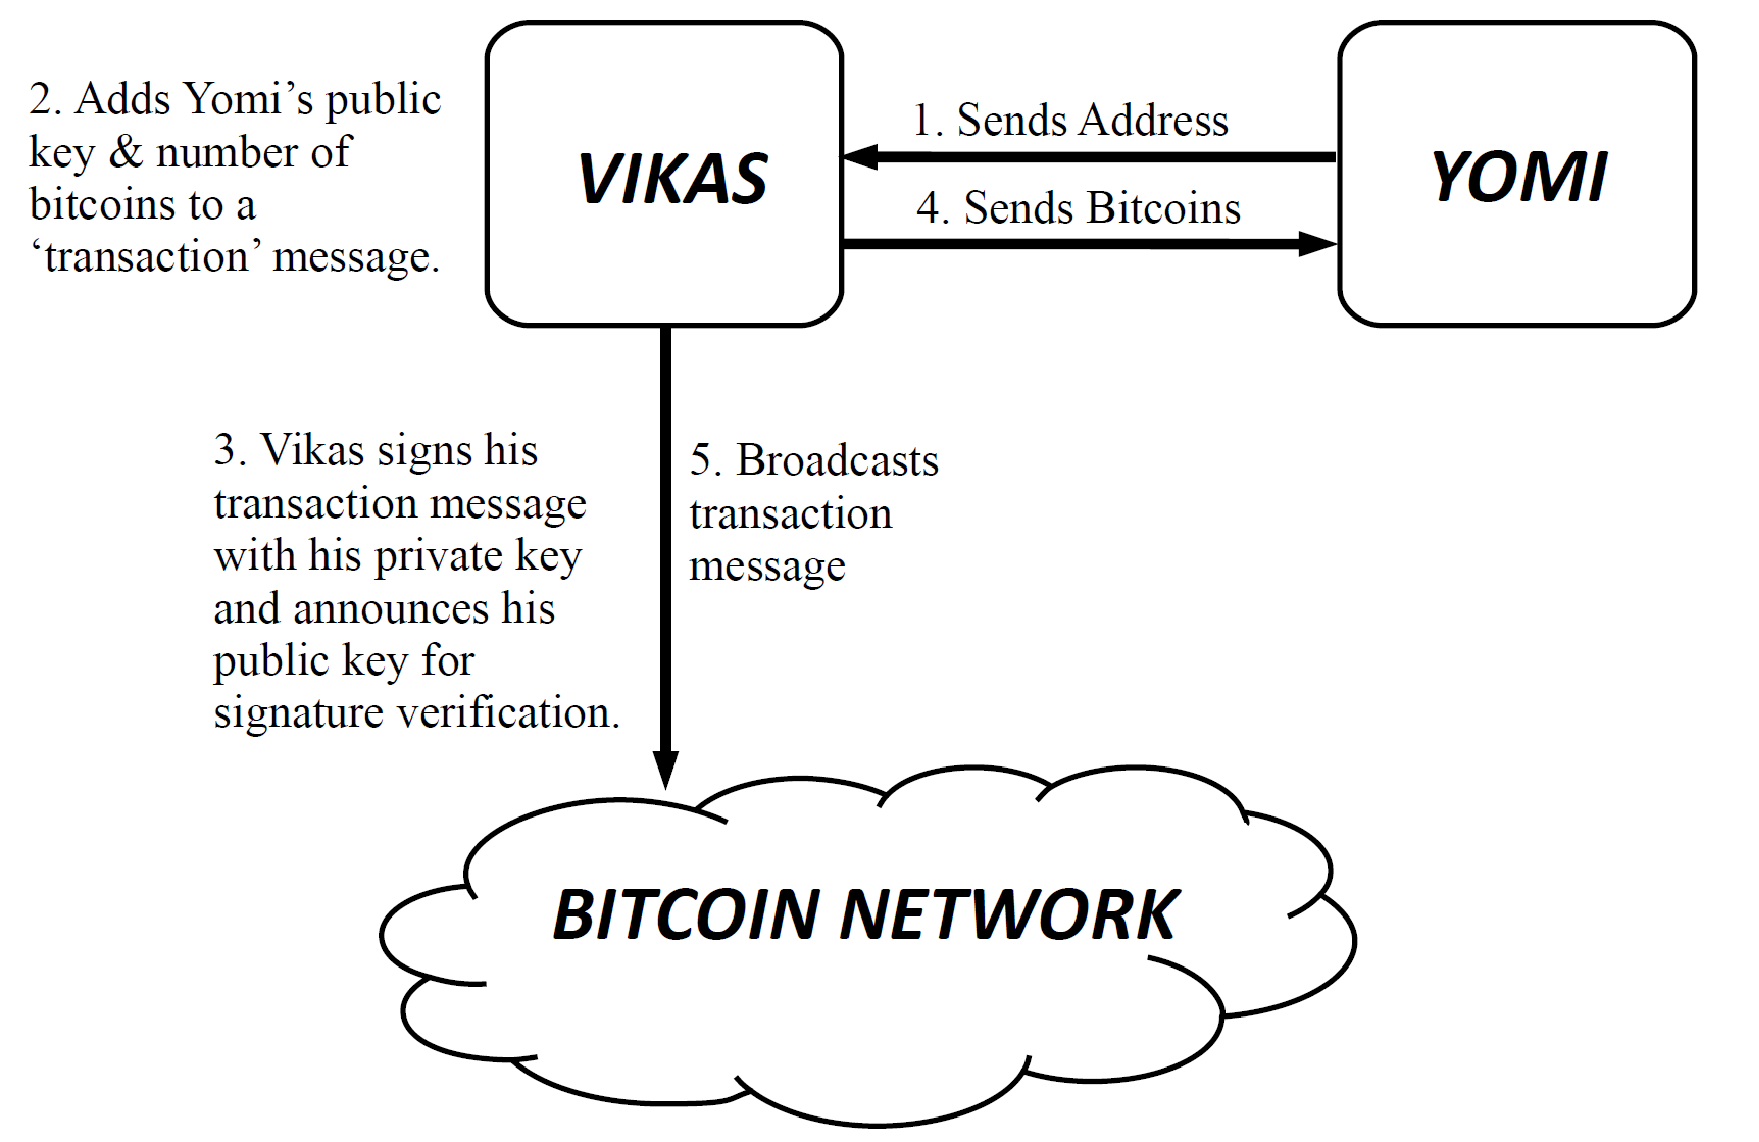
\epsfig{file=Figures/bitcoin_network.pdf, width = \columnwidth}
	\end{center}
	\vspace{-1ex}
	\caption{ Working model of Bitcoin Network 
		\label{Working of Bitcoin Network}}
	\vspace{-4ex}
\end{figure}

\section{Motivation and Scope of the Project}
When a block is getting validated over the network, a protection mechanism is used so that no illegal blocks can be added to these transactions by any form of malicious attempt. A proof of work function is added to each block to ensure its validity. Hashcash is such a proof of work function that is used by bitcoin network and it uses two iterations of SHA-256 algorithm ~\cite{SHA-256}for it's implementation. Just like any other hash function it encrypts data of any arbitrary size into a fixed sized data. If even one bit of the input data is modified, it generates a completely different hash value.
However, bitcoin theft has been documented on several
occasions. There were instances when the bitcoin exchanges
have shut down taking the client’s bitcoins with them. It is
thus extremely important for a strong encryption algorithm to
secure the bitcoin framework. Of late many leading organi-
zations have started accepting bitcoins and it has started to
appeal to general masses as well. Hence bitcoin miners are an integral part of the bitcoin community and is critical to the survival and security of the bitcoin network. Their willingness to contribute their computational power to secure transactions are thus rewarded by the bitcoin community. We were hence motivated to implement our own ASIC that could potentially append transactions in the bitcoin network with a good hash rate.   
Eventhough, the ASIC implementation is capable of mining bitcoins, our focus is to implement the hascash function with a pre-defined block\_header.

\begin{algorithm}[hbt]
	
	{
	block\_header = \{ Version + prev\_block + merkle\_root + timestamp + bits \} \\
			nonce = 0, 	hash = 1\\
	target = 0.000123456789\\
	\While{(\textbf{hash} $>$ \textbf{target})}{hash = SHA256(SHA256(nonce + block\_header))
		\\nonce++}
	}
	\caption {Simplification of mining algorithm}
	\label{mining}
\end{algorithm}

\section{Block Header Fields}
Algorithm Table~\ref{mining} depicts the mining algorithm~\cite{FPGA} involved in bitcoin hashing.
The algorithm shown includes several keywords which are as follows: \\
Version - The version of the block. \\
Prev\_block - Hash value of the previous block. \\
Merkle\_root - hash value of the merkle root of the current block i.e,hash value of the transactions in the current block. \\
Timestamp - current time in seconds after 1970-01-01 T 00:00 UTC. \\
Bits - Number of bits of nonce used to meet the target.


\section{Design Approach}
The core design implementation in the project is of the encryption algorithm SHA-256  Figure~\ref{SHAblockdiagram}, which consists of message packing, scheduling, constant storage, and core math compression. Based on the traditional approach for implementation of the compression technique, we are estimating a gate count close to 120,000 per compression block. The total area over a $0.6\mu$m process technology is being approximated at $0.6nm^2$~\cite{area1,area2}. 


\subsection{Message padding and parsing}
Let's consider a message $M$ of length $L$ bits as input. The message is appended with bit '1' at the end of the message and the resulting data is padded with '$k$' number of 0's, where '$k$' is the smallest non-negative solution to satisfy $k=448-(L+1)$. The message is padded with zero's until the length of message becomes $448\%512$. The rest $64$ bits is length of the message 'L' appended as a 64-bit binary number, thus resulting in a $512$ bit block. If the message is greater than 55 characters, the spillovers form a new $512$ bit message block. Thus the message M is composed into $N$ $512$ bit blocks which are each denoted by $M(1), M(2), M(3) ... M(N)$. 

\begin{figure}[ht]
	\begin{center}
		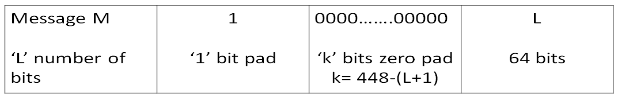
\epsfig{file=Figures/block.png, width = \columnwidth}
	\end{center}
	\vspace{-1ex}
	\caption{A typical padded message 
		\label{padded message}}
	\vspace{-4ex}
\end{figure}

\begin{figure}[ht]
	\begin{center}
		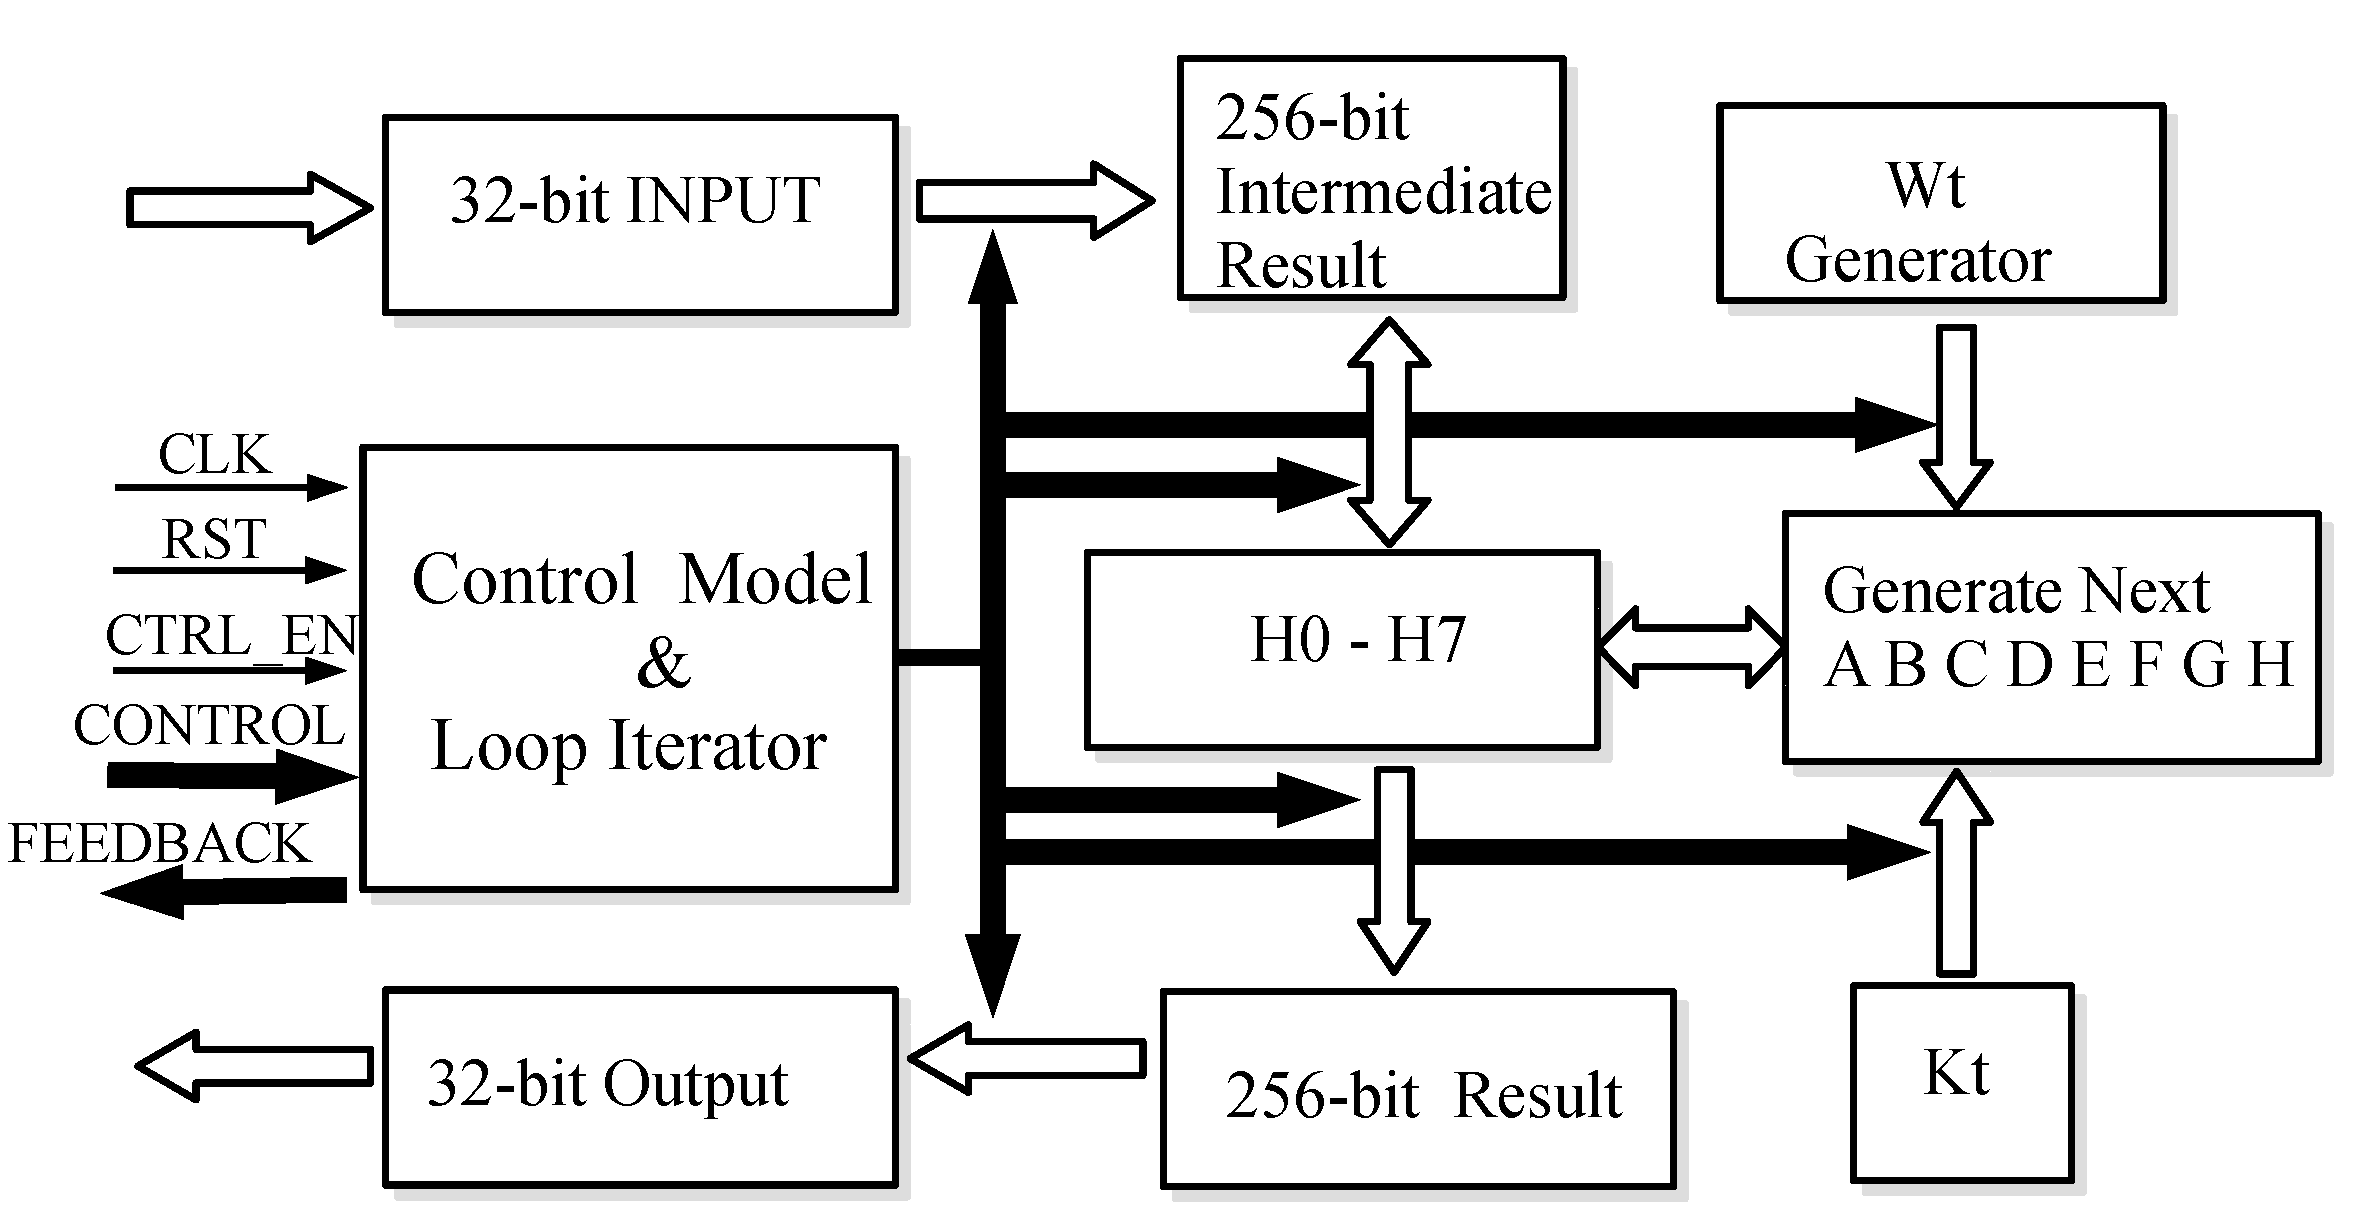
\epsfig{file=Figures/SHA-256.pdf, width = \columnwidth}
	\end{center}
	\vspace{-1ex}
	\caption{Block Diagram of SHA-256. 
		\label{SHAblockdiagram}}
	\vspace{-4ex}
\end{figure}


\subsection{Message expansion, constants, and scheduling}
Each of the $512$ bit $M(i)$ blocks are broken down into 16 32-bit blocks $M_{t}(i)$, where $0 \leq t \leq 15$. The message expansion results in each 512 bit block to get expanded into 64 32-bit blocks denoted by $W(t)$, where $0 \leq t \leq 63$. The message expansion takes place in SHA-256 algorithm using the following set of operations~\cite{FPGA}:

$\sigma_{0} (x) = ROT_{7}(x) \oplus ROT_{18}(x) \oplus SHF_{3}(x) $

$\sigma_{1}(x) = ROT_{17}(x) \oplus ROT_{19}(x) \oplus SHF_{10}(x)$
 
$W_{t} = \begin{cases} 
	M_{t}(i), 0 \leq t \leq 15 \\
	\sigma_{1}(W_{t} - 2) + W_{t} − 7 + \sigma_{0}(W_{t} − 15) + W_{t}-16, 16 \leq t \leq 63  
\end{cases}$

$ROT_{n}(x)$ is a circular rotation of x by n positions to the right.

$SHF_{n}(x)$ is a right shift of x by n positions. 

The expansion also involves pre-defined constants published by NIST. The scheduling involves streaming 32-bit word as input to the subsequent stages of SHA-256 compression.
\begin{figure}[ht]
	\begin{center}
		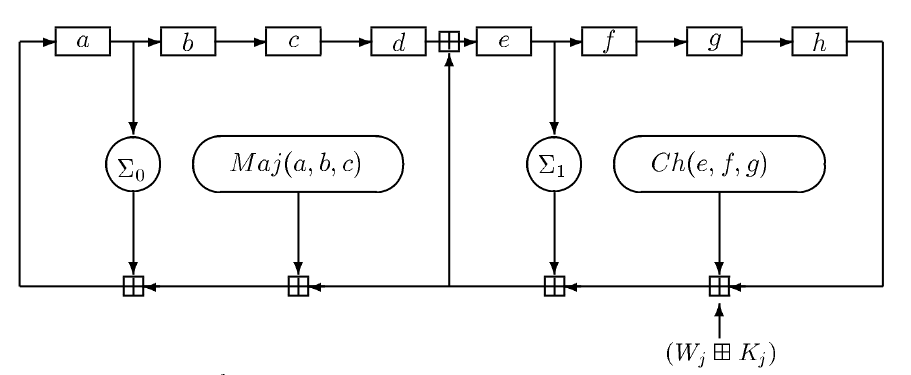
\epsfig{file=Figures/M2.png, width = \columnwidth}
	\end{center}
	\vspace{-1ex}
	\caption{Message Scheduling 
		\label{Message Scheduling}}
	\vspace{-4ex} ~\cite{SHA-256}
\end{figure}
\subsection{Core message Compression}
SHA-256 compression function works on the streamed $W(t)$ block that we get from the expansion stage. In totality, the SHA-256 compression function is computed over a loop on the 512 bit message blocks as follows ~\cite{Newcastle}

$H(i) = H(i-1) + CM(i)(H(i-1))$

Where, C is the SHA-256 compression function.
'+' is word wise mod  $2^{32}$ addition
$H(i)$ is the hash value that is generated for the message $M(i)$.

The compression function uses 8 32-bit variables \textit{A, B, C,.... H}. These are the initial constant values for the first loop of compression and are initialized to the first 32 bits of the fractional parts of the square roots of the first eight prime numbers.~\cite{FPGA} We actually use our block header and encrypt these eight constants. This compression is iterated 64 times using the following operations:

$T_{1} = H + \sum_{1}(E)+ Ch(E,F,G) + K_{t} + W_{t}$

$T_{2} = \sum_{0}(A) + Maj(A,B,C)$
\\where
\\$Ch(x,y,z) = (x AND y) \oplus (\bar{x} AND z)
\\Maj(x,y,z) = (x AND y) \oplus (x AND z) \oplus (y AND z)
\\\sum_{0}(x)= ROT_{2}(x) \oplus ROT_{13}(x) \oplus ROT_{22}(x)
\\\sum_{1}(x)= ROT_{6}(x) \oplus ROT_{11}(x) \oplus ROT_{25}(x)$~~\cite{FPGA}\\The $K_{t}$ inputs are 64 32-bit constants which are initialized to the first 32 bits of the fractional parts of the cube roots of the first 64 prime numbers. \cite{FPGA}
\begin{figure}[ht]
	\begin{center}
		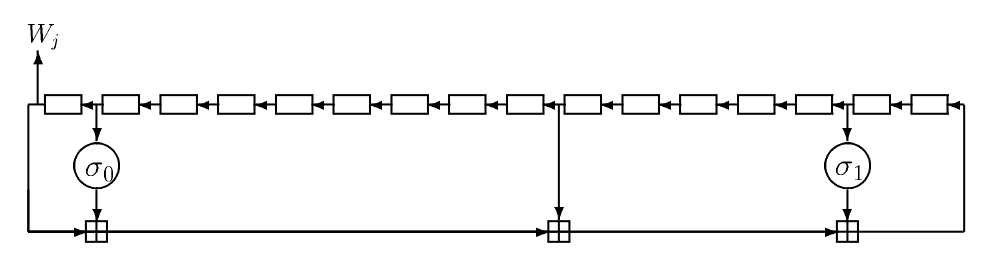
\epsfig{file=Figures/M1.png, width = \columnwidth}
	\end{center}
	\vspace{-1ex}
	\caption{Message Compression
		\label{Message Compression}}
	\vspace{-4ex} ~\cite{SHA-256}
\end{figure}
\\During every $i^{th}$ iteration, $ \\ H=G\\ F=E\\ D=C\\ B=A\\G=F\\E=D+T_{1}\\C=B\\ A= T_{1}+T_{2}$~\cite{FPGA}
\\After 64 iterations of this SHA-256 compression function the immediate hash values are computed. 
\\$H_{0}^{(i)} = A + H_{0}^{(i-1)}$
\\$H_{1}^{(i)} = B + H_{1}^{(i-1)}$
\\$H_{2}^{(i)} = C + H_{2}^{(i-1)}$
\\$H_{3}^{(i)} = D + H_{3}^{(i-1)}$
\\$H_{4}^{(i)} = E + H_{4}^{(i-1)}$
\\$H_{5}^{(i)} = F + H_{5}^{(i-1)}$
\\$H_{6}^{(i)} = G + H_{6}^{(i-1)}$
\\$H_{7}^{(i)} = H + H_{7}^{(i-1)}$ \cite{FPGA}
\\This compression algorithm is computed on all the 512-bit blocks. Suppose there are $N$ 512-bit blocks, the final 256-bit hash output is the concatenation of the hash values of $N^{th}$ block.
\\$H^{N} = H_{0}^{(N)}H_{1}^{(N)}H_{2}^{(N)}H_{3}^{(N)}H_{4}^{(N)}H_{5}^{(N)}H_{6}^{(N)}H_{7}^{(N)} $ \cite{FPGA}


\subsection{Overview of Bitcoin mining implementation}
The block header is used to encrypt the constants specified by NIST. Our block header consists of 640 bits- Version[31:0], Previous hash value[255:0], Merkle Tree [255:0], Timestamp[31:0], Difficulty bits [31:0], Nonce[31:0].
\\Bitcoin mining requires finding the value of the cryptographic nonce so that the hash value is within a certain range for that block. The nonce value is such that the double SHA-256 hash value of the block is less than a given $threshold$ value. This $threshold$ value varies over time as a function of the difficulty bits that is adjusted by the network itself such that a valid transaction block is added to the network approximately every ten minutes. This means that a valid hash of hash solution, that matches the given $threshold$, is found every ten minutes. The first miner who finds the valid nonce value broadcasts it throughout the bitcoin network and is thus rewarded. 
\\Nonce is the last 32 bits of the block header. As mentioned earlier the nonce value needs to be changed until the double hash of the block meets the given threshold, thus nonce is the only changing bits in the entire 640 bits block header.Out of these 640 bits, the first 512 bits do not need padding as these bits are fixed for a particular hash computation. These bits can itself form the first 512-bit block and can directly continue to the parsing stage. The rest 128 bits of the 640-bit header are padded to produce the second 512-bit block. The first 512 bits do not change across nonce iterations hence it's hash can be precomputed. This 256-bit hash value of the first block is parsed into 8 32-bit values and are used to encrypt the second block instead of the the given $A, B, C,....H$ values. The hash output of the second block is hashed again using SHA-256 which gives the final hash value. This final hash value is checked against the $threshold$.
\\The constituent core blocks (Figure ~\ref{ourimplementation}) are developed in verilog HDL with each operation register size being 32 bit DWORD. Every RTL core is validated through a individual verilog testbench to get a block level debug view. The final top level test bench has our module implementation output compared against a SHA-256 software model implementation. All the necessary basic cells and gates for the project is taken from those developed in the group project library. 

\begin{figure}[ht]
	\begin{center}
		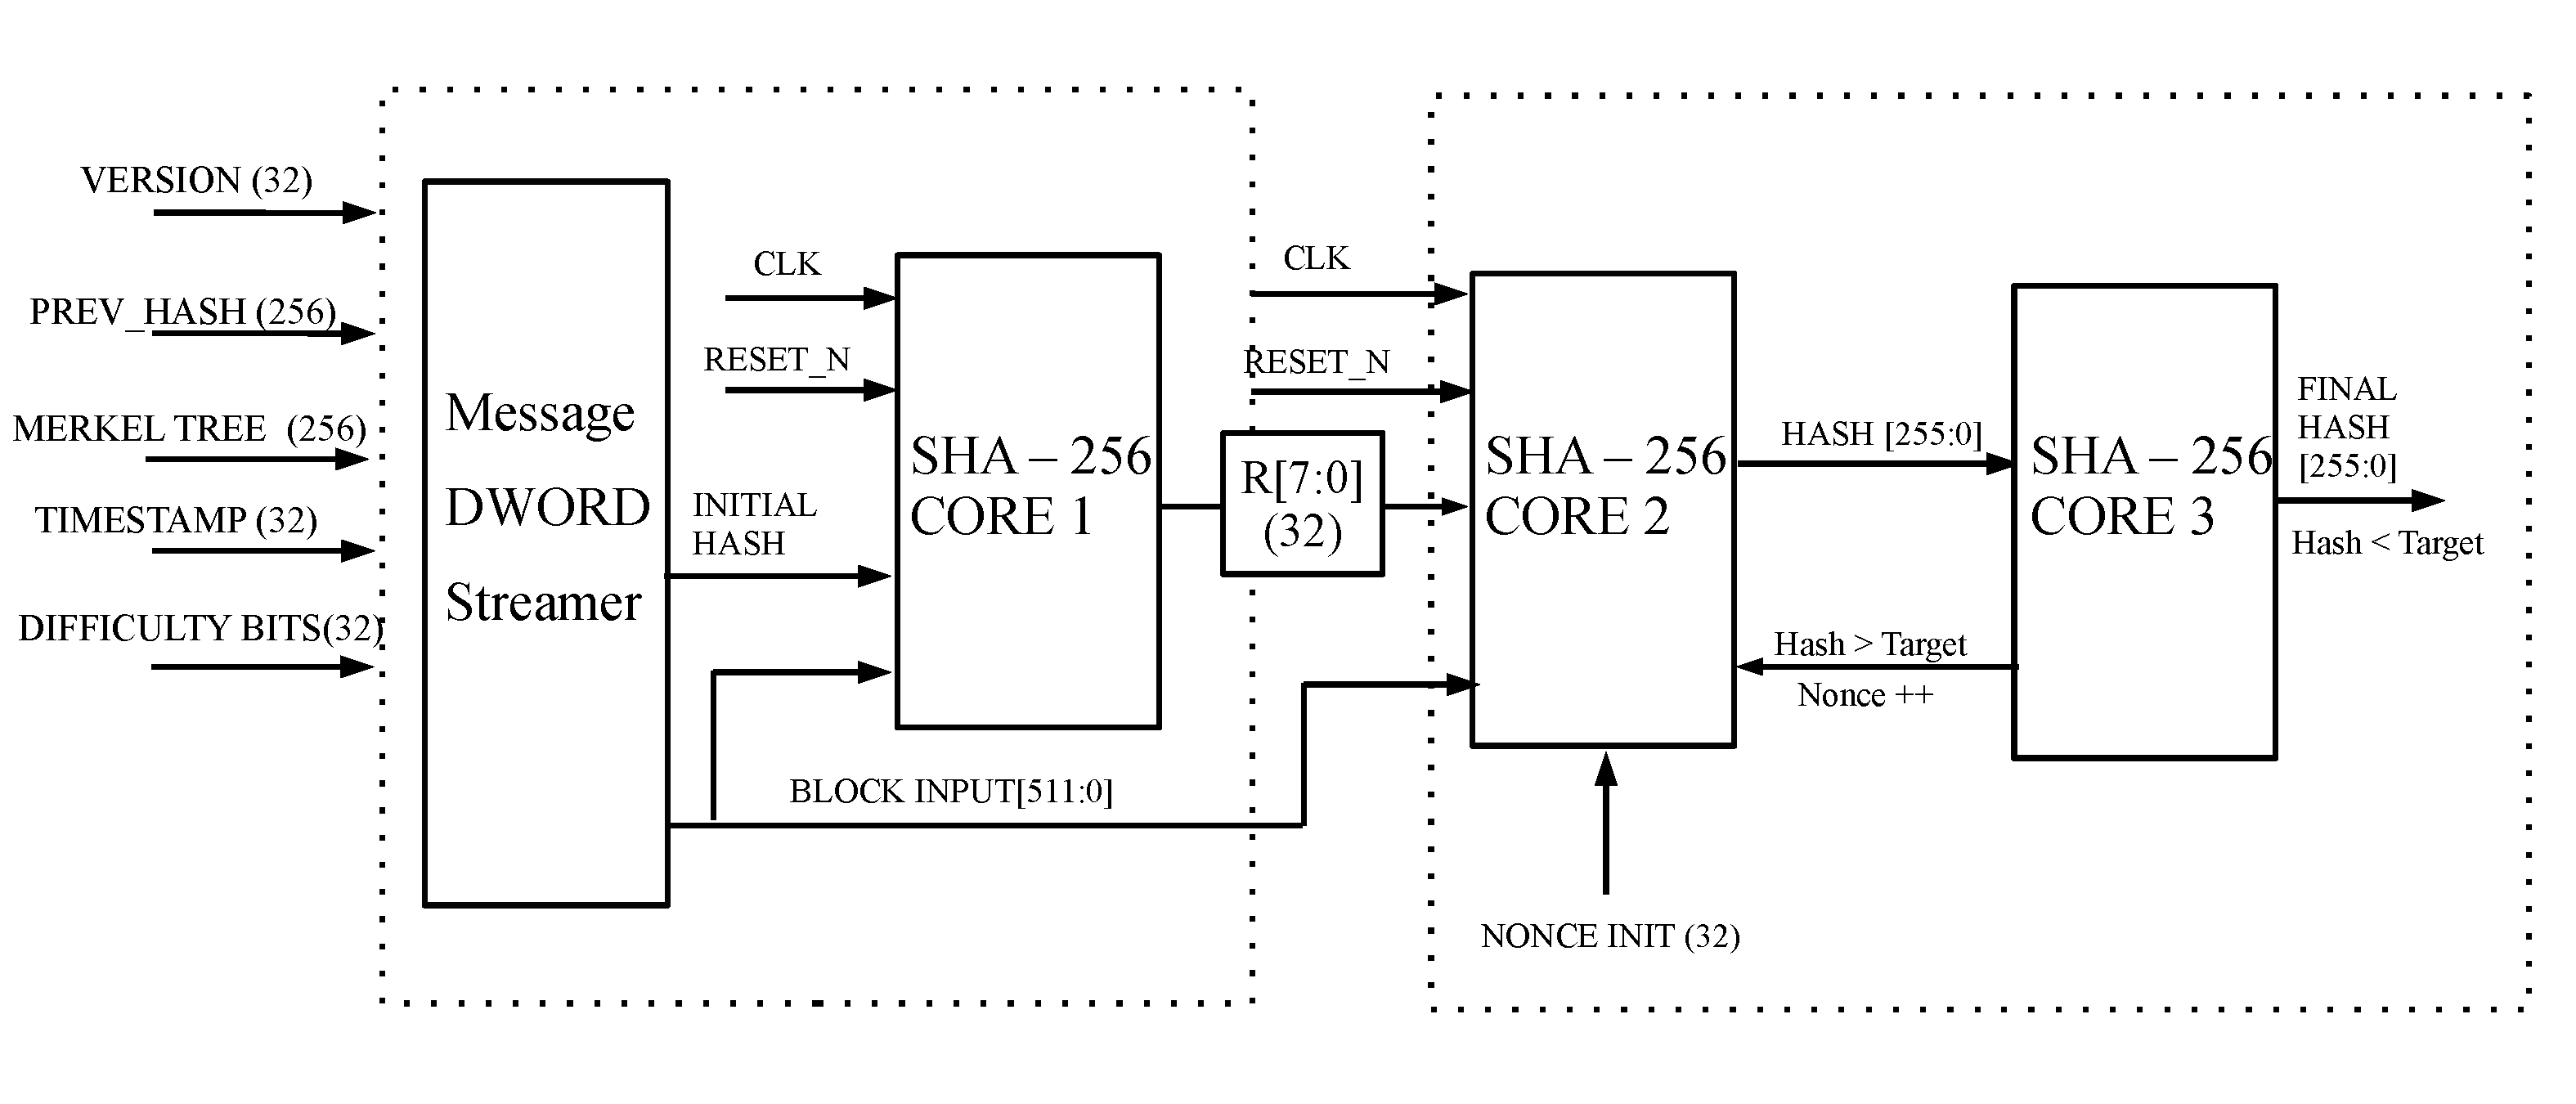
\epsfig{file=Figures/bitcoin.pdf, width = \columnwidth}
	\end{center}
	\vspace{-2ex}
	\caption{Our Bitcoin Implementation. 
		\label{ourimplementation}}
	\vspace{-2ex}
\end{figure}

To reduce the layout area imprint for block operations, we have also developed some hand-written, optimized DWORD gates. 


\section{ASIC Implementation}
Our ASIC is implemented using Verilog and synthesized using Synopsys Design Compiler. The development of the ASIC core involved building RTL cores for the every function implementation which are then verified using individual verilog testbenches.
\subsection{RTL Approach}
We define two cores for our Verilog design, one of which performs iterations and the other core to carry out all our ALU computations. 
\\The SHA-256 expansion stage performs two different types of operations based on the value of $t$ which is the the value of the iteration as discussed earlier. The $Iterator$ core that we designed takes 32-bit message input $M{t}(i)$ from the parsing stage and computes $W_{t}$. The value of $W_{t}$ remains the same as the input $M{t}(i)$ for the first 16 iterations that is for $t$ ranging from 0 to 15. The $W_{t}$ for $t$ values ranging from 16 to 63, is computed using rotating and shifting functions on the previous $W_{t}$ values generated for every iteration. Our $Iterator$ core uses $genvar$ for implementation of these two $for$ loops.$Genvar$ is a variable used in generate-for loop in verilog and stores positive integer values. The $Iterator$ calls functions that are defined in our $ALU$ core.
\\The second core that performs ALU operations defines separate modules for each functional operation. This core computes the values of $ \sigma_{0}, \sigma_{1}, Maj, Ch $ functions. It basically performs the Rotation, Shifting, XOR, AND operations required for those functions. These operations are called from the $Iterator$ core. Thus the functions defined here in the $ALU$ core are used in the $Iterator$ core for each iteration in the SHA-256 Algorithm.
\subsection{Testbench Approach}
Each of our RTL cores are validated using Verilog testbenches to get a debug view of each and every stage of the SHA-256 Algorithm and also the entire Bitcoin mining double hash. Our testbench has a block header input, checks first the 256-bit hash computed for that block with the actual hash value for that block. This validates a single working SHA-256 hash core that we implemented. A testbench also checks the double hash for a 640-bit block header with a working software implementation of a bitcoin hash generator.
We checked if our SHA-256 core is working by using several input block headers. As an example, if our input message to the SHA-256 core given is $abc$, we get the hash of this input as: \\ba7816bf 8f01cfea 414140de 5dae2223 b00361a3 96177a9c b410ff61 f20015ad
\\We verified this output through a testbench with the actual SHA-256 hash of $abc$.
This computation of hash involved multiple steps. At the first, each of a, b and c was converted into their 8-bit ASCII value.
\\8 bit ASCII of a: 01100001
\\8 bit ASCII of b: 01100010
\\8 bit ASCII of c: 01100011
This 24 bit word was now padded with a '1' and 423 '0's followed by '24' in a 64 bit binary. The resulting padded message was thus 512 bits.This 512-bit message was broken down into 16 32-bit DWORDS which were then expanded to form 64 32-bit DWORDS using message expansion as discussed above. The expanded message is then compressed using the SHA-256 compression function, thus producing the hash value.
Once we verified the working of one SHA-256 core, our double hash digest was also verified using the testbench.
\section{Hardware Implementation} 
The bitcoin mining double hash that we implemented using behavioral verilog was synthesized using the library that we built. This library consists of basic cells AND, AOI, 4X\_Buffer, 8X\_Buffer, Ch function(Choosing) , D- FLIPFLOP, Filler cell, Inverter, 4X\_Inverter, 8X\_Inverter, Maj function(Majority), NAND, 2X\_NAND, NOR, TIEHIGH, TIELOW, XOR, XNOR.
\\The library was first characterized using the Signal Storm Tool in Cadence to generate the $.db$ file and the Abstract tool was used to generate a $.lef$ file. This $.db$ file was used in Synopsys Design Compiler to synthesize the structural verilog code from the behavioral verilog code. We performed place and route using the synthesized verilog file and the generated $.lef$ file with a row spacing of 60 microns and density of 10\%. Due to large amount of parallel operations and hence greater number of wires, there were many violations.To reduce these violations occurring from congestion, we prevented the tool from flipping the cells that it does to reduce area. Finally this was taken back to Virtuoso for Design rule and Schematic checks. This resulted in an ASIC having an area of XX and a gate count of XX with yy AND, yy AOI, 4X\_Buffer, 8X\_Buffer, Ch function(Choosing) , D- FLIPFLOP, Filler cell, Inverter, 4X\_Inverter, 8X\_Inverter, Maj function(Majority), NAND, 2X\_NAND, NOR, TIEHIGH, TIELOW, XOR, XNOR.
\section{Results}
\section{Further Optimizations Proposed}
After having read and reviewed research papers based on Bitcoin mining and SHA-256, we intend to incorporate the optimizations explicitly stated in those papers to enhance our implementation of a bitcoin hash ASIC. 
\\~\cite{} mentions that bitcoin mining is a suitable candidate for approximate computing. The parallel nature of bitcoin mining can be exploited to increase bitcoin mining profits by replacing circuits with their approximate versions and allowing a Better than Worst-Case (BTWC) operation. Approximations give greater mining profits even when the hash computed is incorrect, as any wrong solution gets invalidated by other bitcoin miners in the network. This optimization trades off reliabity with delay and area. Using approximate circuits reduces delay which in turn increases frequency and overall throughput. It also reduces area, which can be used for incorporating more hashing cores on the ASIC. From the results reviewed from the paper it is seen that there's a 30\% increase in mining profits using approximate adder $KSA_{16}$(Kogge Stone Adder) compared to their accurate counterparts like $CLA$ (Carry-lookahead adder) or $KSA_{32}$. 15\% of the 30\% increased profit is due to functional approximation that is using approximate cirtuits and the other 15\% is derived from operational approximation. Operational approximation involves reducing guard bands, running the cicuit at a negative timing slack, BTWC operation and allowing ocassional timing violations. We plan to try and design the $KSA_{16}$ adder for out bitcoin miner in order to increase mining profits.  

\section{Conclusion}
